\section{Desenvolvendo a \emph{API} \emph{Web}}
Para o desenvolvimento da \emph{API}, escolheu-se a linguagem \emph{Python}, por sua clareza, 
e sua alta produtividade, que é crucial no processo de prototipação. Em conjunto com \emph{Python}, 
o \emph{micro framework web} \emph{Flask} também foi escolhido. Justifica-se essa escolha pela
inerente simplicidade, clareza e produtividade do \emph{framework}. 

Antes de podermos modelar recursos para a \emph{API},
estudaram-se quais dados eram necessários para os casos de uso propostos. Este estudo gerou um 
\emph{MER}, modelo entidade relacional, que relacionava todas as entidades do sistema. A partir 
do diagrama gerado, criou-se um conjunto de ``\emph{models}'' para representar estas entidades. A classe 
que possibilitou a criação destes \emph{models} provém da \emph{ORM} que abstrai bancos 
relacionais chamada \hyperref[link:sqlalchemy]{\emph{SQLAlchemy}}. \hyperref[link:sqlalchemy]{\emph{SQLAlchemy}}
é uma biblioteca estável com mais de treze anos de maturidade,
mas que continua sendo a escolha padrão dos desenvolvedores.

Optou-se por utilizar \hyperref[link:postgresql]{\emph{PostgreSQL}}.
A escolha foi feita por se tratar de um sistema 
gerenciador de banco de dados relacional de código aberto e por este ser referência em 
desempenho e funcionalidades.

No mapeamento do \emph{MER}, previamente esboçado, em classes utilizou-se a biblioteca 
de visualização \hyperref[link:eralchemy]{\emph{ERAlchemy}}. \hyperref[link:eralchemy]{\emph{ERAlchemy}} é capaz de gerar 
diagramas \emph{MER} de forma automática a partir das classes modelo ou de uma conexão com o banco de dados. 
Tal ferramenta se provou excepcionalmente útil pois permitiu o desenvolvimento incremental e iterativo das 
classes modelo e garantiu que o modelo conceitual fosse implementado sem divergências. A \fref{fig:mer} mostra 
o modelo entidade relacional do sistema, gerado a partir da ferramenta.

Para que nosso sistema fosse capaz de armazenar submissões de alunos de forma confiável,  
um serviço de intervalos de  armazenamento, traduzido do inglês \emph{Bucket Storage}, se 
fez necessário. Um intervalo de armazenamento nada mais é que uma abstração de provedores 
de computação em nuvem para oferecer armazenamento de objetos. Uma das grandes vantagens associadas 
a este tipo de serviço é o baixo custo por \emph{gigabyte}, além de sua alta escalabilidade, tanto 
 um aumento no volume de dados armazenados, quanto na velocidade recuperação destes.
O provedor de computação em nuvem escolhido foi a \hyperref[link:gcp]{\emph{Google Cloud Plataform}}.


A alternativa a adotar um serviço de armazenamento por intervalos seria armazenar arquivos 
diretamente no banco de dados, o que traria um impacto na performance do mesmo, já que \emph{SGBD}s não são otimizados para
este tipo de dado. 

Modelaram-se recursos seguindo o estilo arquitetural \emph{REST}. Coleções e documentos
de exercícios, turmas, tópicos, entre outros recursos foram implementados, e um 
recurso do arquétipo \emph{controller} foi necessário para prover autenticação a interface por 
meio do fluxo de concessão do código de autorização. Também disponibilizou-se uma rota para \emph{health check}, 
que permite que uma sonda externa consulte se a aplicação continua funcionando adequadamente. Caso esta não esteja, 
envia-se um sinal para que um novo contêiner da aplicação seja iniciado e o tráfego é redirecionado a ela. 

Para que não seja necessário que professores criem um banco de exercícios do zero, um ``conector'' foi 
implementado para a plataforma \emph{exercism}, em que seus exercícios são extraídos e guardados no banco 
de dados. A implementação aborda apenas duas linguagens \emph{Python} e \emph{Rust}, mas 
pode ser facilmente estendido para outras linguagens, dado que se informe a estrutura de arquivos 
que os exercícios daquela linguagem são armazenados.

Também foi configurado uma plataforma de \emph{CI/CD} para o projeto. A toda nova versão enviada 
ao repositório remoto do sistema de controle de versões, uma tarefa rodava a ferramenta \emph{autopep8}
que checava se o código \emph{commitado} era sintaticamente válido e não seguia más práticas. 
Caso o código fosse reprovado na tarefa anterior, este não poderia ser aprovado e mesclado 
na \emph{branch} principal de desenvolvimento. Se a contribuição passar na verificação e 
depois de revisão for aceita, uma tarefa para lançamento da nova versão é disparada automaticamente, 
       que coloca uma nova versão no ar. A plataforma de \emph{CI/CD} empregada foi o 
       \hyperref[link:actions]{\emph{Github Actions}} e 
       as novas versões eram colocadas no ar através da \emph{Platform as a Service} do \emph{Google}, 
       \hyperref[link:appengine]{\emph{AppEngine}}.  \\ 
       O \Aref{capitulo:cicd} conceitua com mais detalhes o que é integração e  entrega contínua .



\section{Desenvolvendo a CLI}
O desenvolvimento da \emph{CLI} foi feito na linguagem \emph{Rust}, utilizando 
a biblioteca \emph{StructOpt}.  \emph{StructOpt} é uma biblioteca que permite construção 
de interfaces por linhas de comando a partir da anotação de macros em \emph{structs} ou 
\emph{enums}. Com uma simples anotação ganha-se um \emph{parser} dos comandos e mensagens 
que instruem o usuário como utilizar sua \emph{CLI}. Também utilizou-se a biblioteca \emph{reqwest} que fornece um cliente \emph{HTTP} que abstraí
a construção de requisições e facilita o consumo de respostas.

\section{Desenvolvendo a interface}
A interface foi desenvolvida utilizando \emph{Javascript}, \emph{CSS} e \emph{HTML}. Como 
desejávamos uma plataforma que fosse bastante interativa, uma \emph{single page application} 
foi implementada, utilizando a tecnologia \hyperref[link:react]{\emph{React}}.
Seguiu-se o \emph{design system} chamado 
\emph{Material Design} por ser bastante intuitivo para novos usuários. A biblioteca \emph{Material-UI} 
forneceu vários componentes que serviram de base para os componentes customizados. A comunicação com a 
\emph{API} foi feita utilizando o cliente \emph{HTTP} \hyperref[link:axios]{\emph{axios}} e 
os dados são persistidos numa \emph{store} local, utilizando o gerenciador de estados \emph{Redux}.

\begin{sidewaysfigure}[htpb]
    \centering
    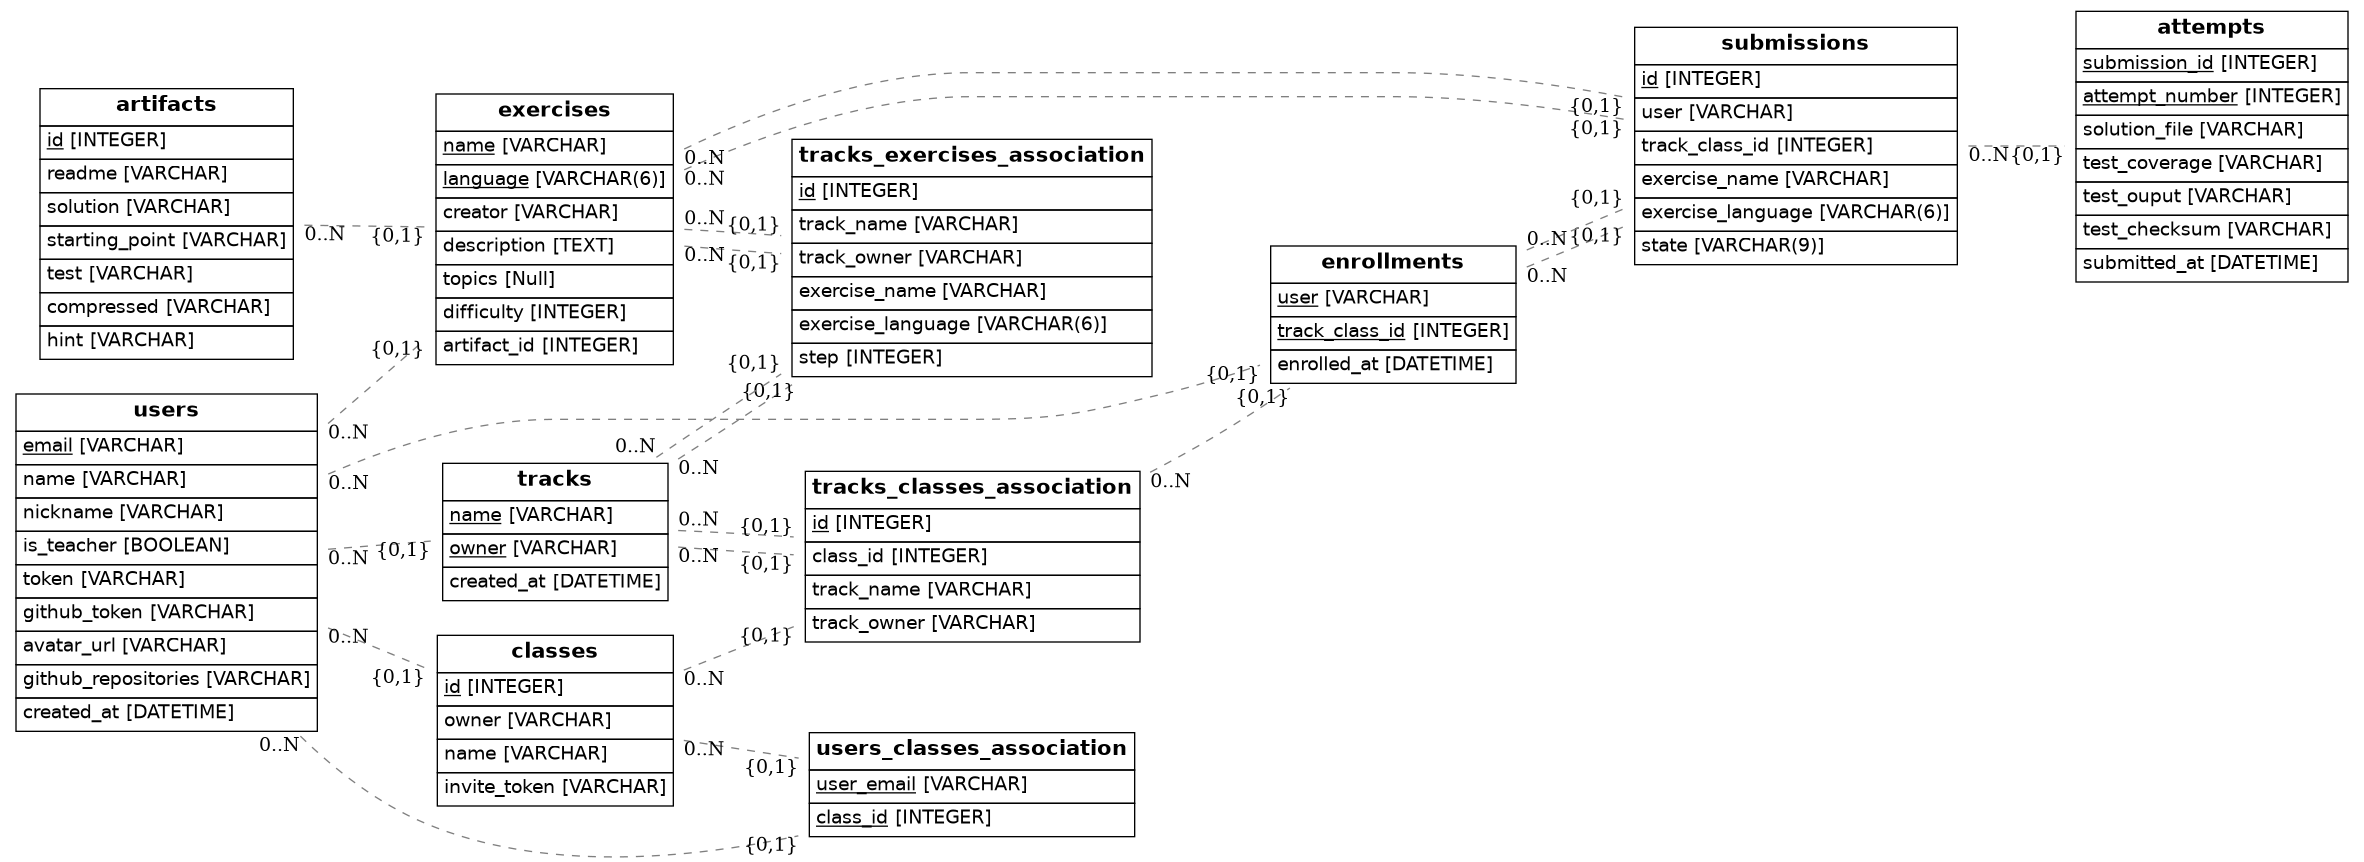
\includegraphics[width=\linewidth]{images/db_schema}
    \caption{Modelo entidade relacional gerado a partir da ferramenta \hyperref[link:eralchemy]{\emph{ERAlchemy}}.}\label{fig:mer}
\end{sidewaysfigure}